\documentclass{article}
\usepackage[utf8]{inputenc}
\usepackage[francais]{babel}
\usepackage{array}
\usepackage{graphicx}
%\usepackage{fullpage}
\usepackage[svgnames]{xcolor}
\usepackage{color}
%\usepackage{fourier}
\usepackage{pifont}

\newcommand*{\rotrt}[1]{\rotatebox{90}{#1}} % Command to rotate right 90 degrees
\newcommand*{\rotlft}[1]{\rotatebox{-90}{#1}} % Command to rotate left 90 degrees

\newcommand*{\titleBC}{\begingroup % Create the command for including the title page in the document
\centering % Center all text

\def\CP{\textit{\Huge Rapport Projet Ontologies et Web sémantique}} % Title

\settowidth{\unitlength}{\CP} % Set the width of the curly brackets to the width of the title
\textcolor{FireBrick}{\CP} \\[\baselineskip] % Print title
{\color{Grey}\Large "Ontologie des musées et application TrouverUnMusée.fr"} \\
% Tagline or further description
\endgroup}

\definecolor{lg}{rgb}{0.9,0.9,0.9}

\let\oldv\verbatim
\let\oldendv\endverbatim

\def\verbatim{\setbox0\vbox\bgroup\oldv}
\def\endverbatim{\oldendv\egroup\fboxsep0pt \colorbox[gray]{0.9}{\usebox0}\par}

\setlength\parindent{0cm}

%%%% Le Document %%%%

\begin{document}

\begin{table}[h]
    \begin{center}
    \begin{tabular}{ >{\centering\arraybackslash}m{1.5in} >{\arraybackslash}m{4in} }

    \vspace{5mm} 
\includegraphics[width=2cm]{logo.png} & \vspace{9mm} Ce projet
    a été réalisé dans le cadre du cours de d'Ontologies et Web
    sémantique du Master 2 Pro. GI. par \textbf{Johan GIRARD}, \textbf{Pierre
    ODIN} et \textbf{Abdourahamane TOURÉ}.

  \end{tabular}

  \label{tabular:UKJPNdata}
  \end{center}
\end{table}

\hrule\hrule

\vspace{1.5cm}

\titleBC

\vspace{1cm}

\section{Partie 1 : L’ontologie et les données}

\subsection{Jeu de données}

Le fichier de données sur lequel nous nous sommes basé pour créer notre
ontologie et notre application contient la \textbf{liste des Musées de France
en 2012}. Ces données sont disponibles sur le site \texttt{data.gouv.fr}
(à l'adresse suivante :
\textit{https://www.data.gouv.fr/fr/datasets/liste-et-localisation-des-musees-de-france/}).
Ce fichier contient une liste d'environ 1200 musées en indiquant pour chacun
d'entre eux différentes informations comme son  nom, sa localisation, ses
horaires d'ouverture, etc\ldots

\subsection{L'ontologie (protege)}

L'entité principale de notre ontologie est un \texttt{Musée}. Elle est
équivalente à l'entité \texttt{Museum} de l'ontologie \texttt{schema}
(\texttt{http://schema.org/}). Les entités suivantes permettent de caractériser
un \texttt{Musée} : 
\begin{itemize}
  \item \texttt{Adresse} qui est liée aux entités \texttt{Ville},
\texttt{Département} et \texttt{Région}. Ces entités sont
équivalentes a des entités de l'ontologie \texttt{igeo}
(\texttt{http://rdf.insee.fr/def/geo\#}) et sont des sous-classe de l'entité
\texttt{Localisation}.
  \item \texttt{Thème}
  \item \texttt{SiteWeb} (équivalente à
l'entité \texttt{WebSite} de l'ontologie \texttt{schema})
\item \texttt{HoraireOuverture} , \texttt{OuvertureNocture}
, \texttt{FermetureAnnuelle} , \texttt{DateRéouverture} (un musée ayant une date
de ré-ouverture est un musée actuellement en fermeture prolongée). Ces entités
sont des sous-classe de l'entité \texttt{Période}.
\end{itemize}

\vspace{0.3cm}

L'entité \texttt{MuséeAvecThème} est une sous-classe de \texttt{Musée} qui
regroupe les musées ayant un thème défini. L'entité \texttt{MuséeDisponible} est
une autre sous-classe de \texttt{Musée} qui regroupe les musées qui ne sont
pas actuellement en fermeture prolongée.

\vspace{0.3cm}

Toutes les propriétés sont \texttt{Asymmetric} et \texttt{Irreflexive}.
Certaines propriétés sont \texttt{Fonctional} et d'autres sont
\texttt{Inverse Fonctional} (respectivement notées \texttt{(F)} et \texttt{(IF)}
dans le schéma de l'ontologie ci-après).

%\paragraph{\starredbullet}
Nous avions également complété l'ontologie avec une
propriété nommée \texttt{estVilleDeLaRégion} qui utilisait l'option
\texttt{SubPropertyOf (Chain)} mais nous avons dû la supprimer car elle
bloquait l'utilisation du raisonneur.

\newpage

Le schéma en trois parties de l'ontologie des musées réalisée est le suivant :

\begin{center}
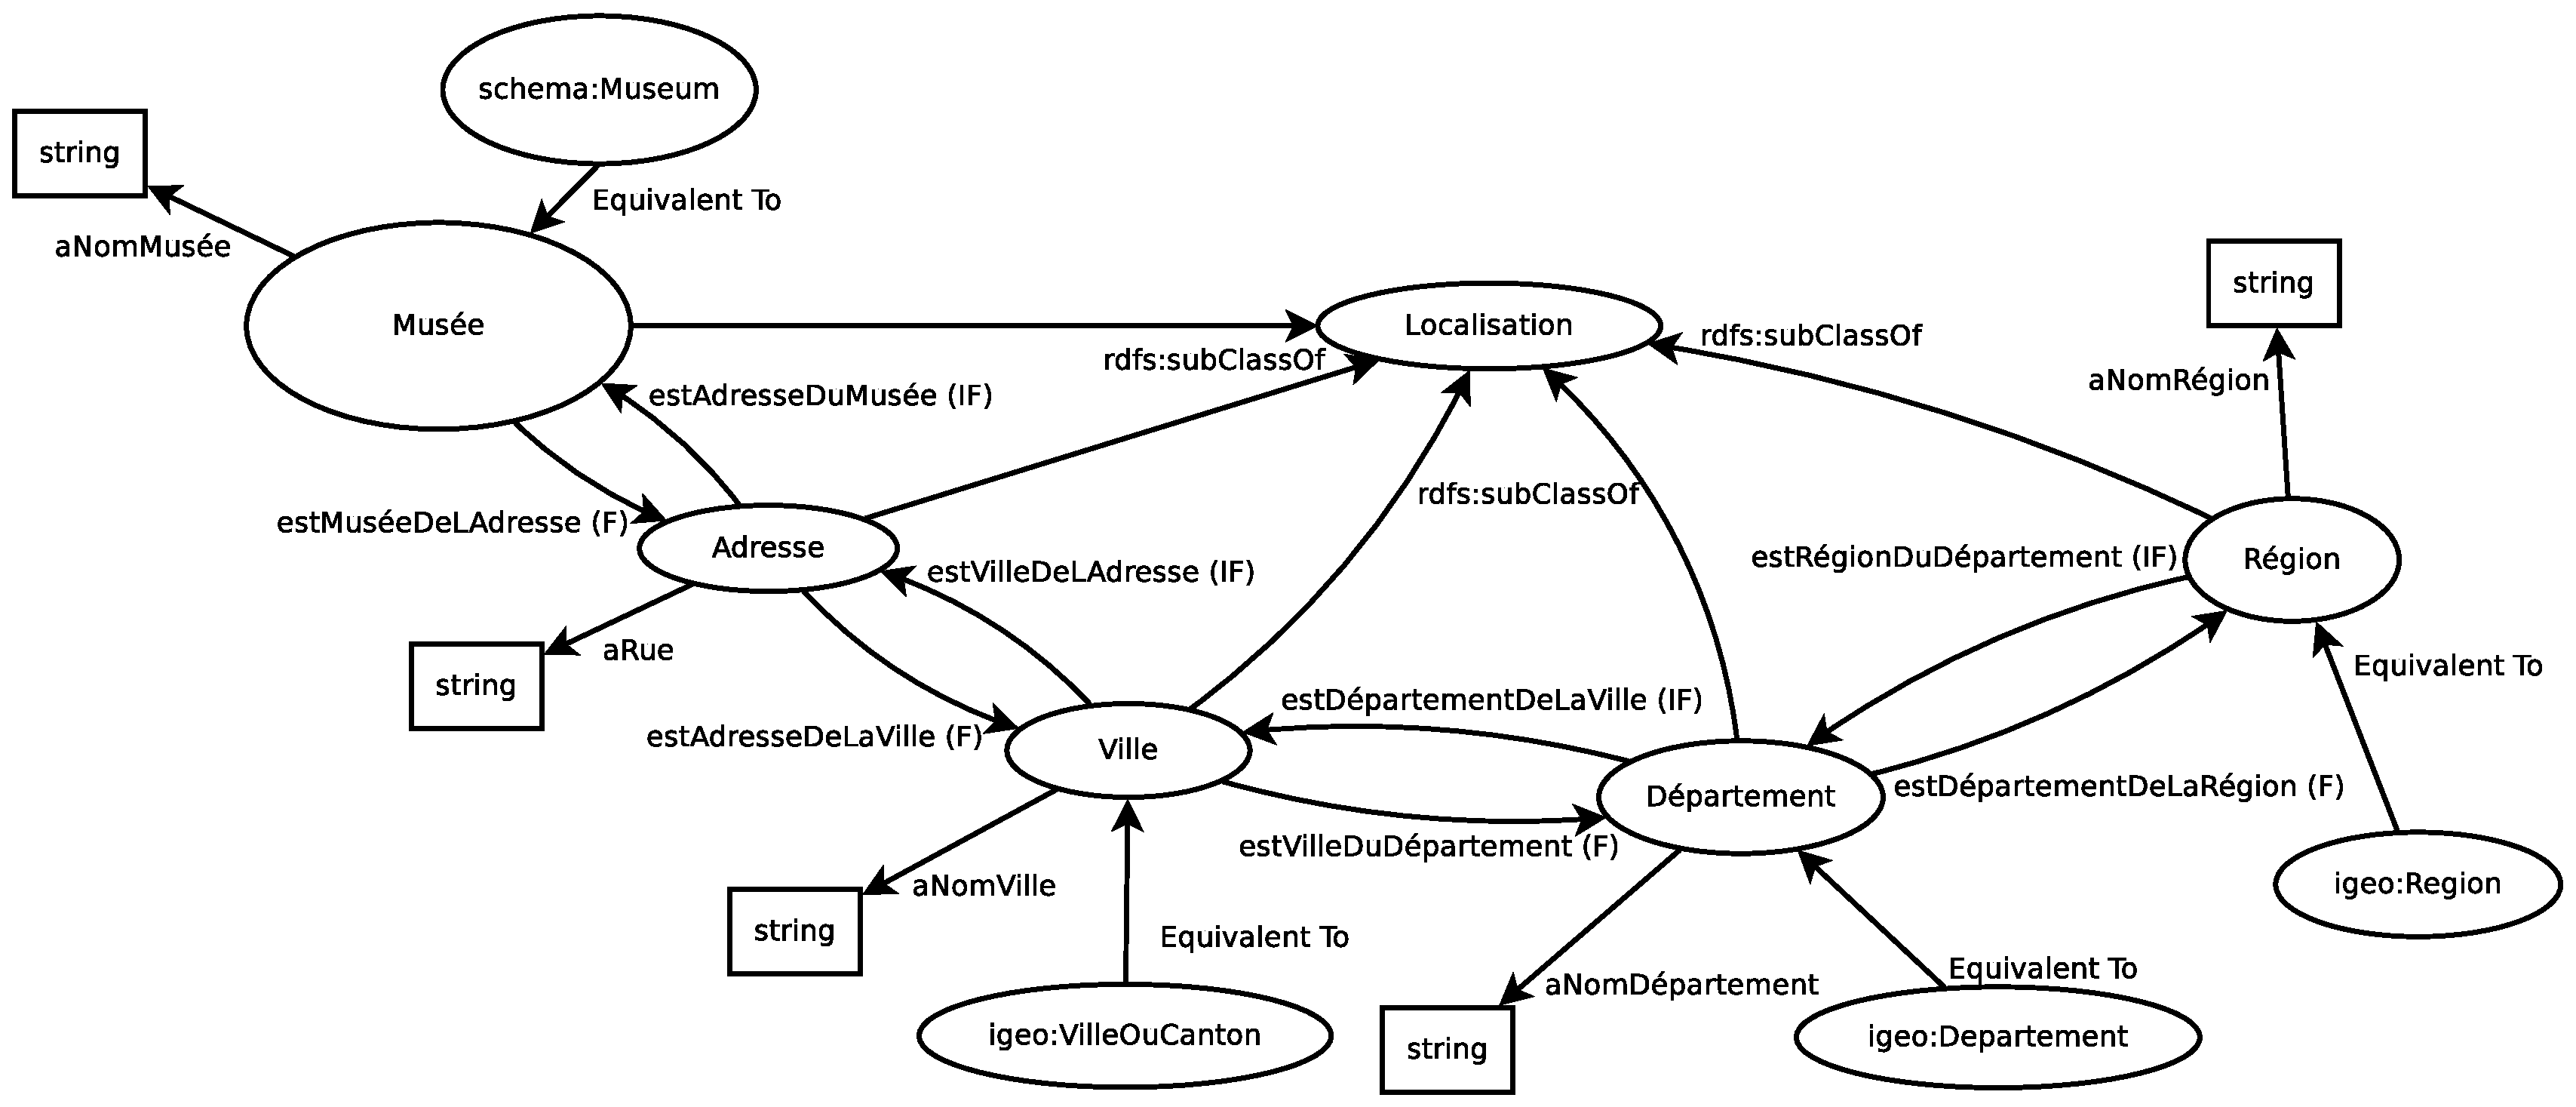
\includegraphics[width=16cm]{Diagramme1.eps}
\end{center}
\vspace{0.3cm}
\begin{center}
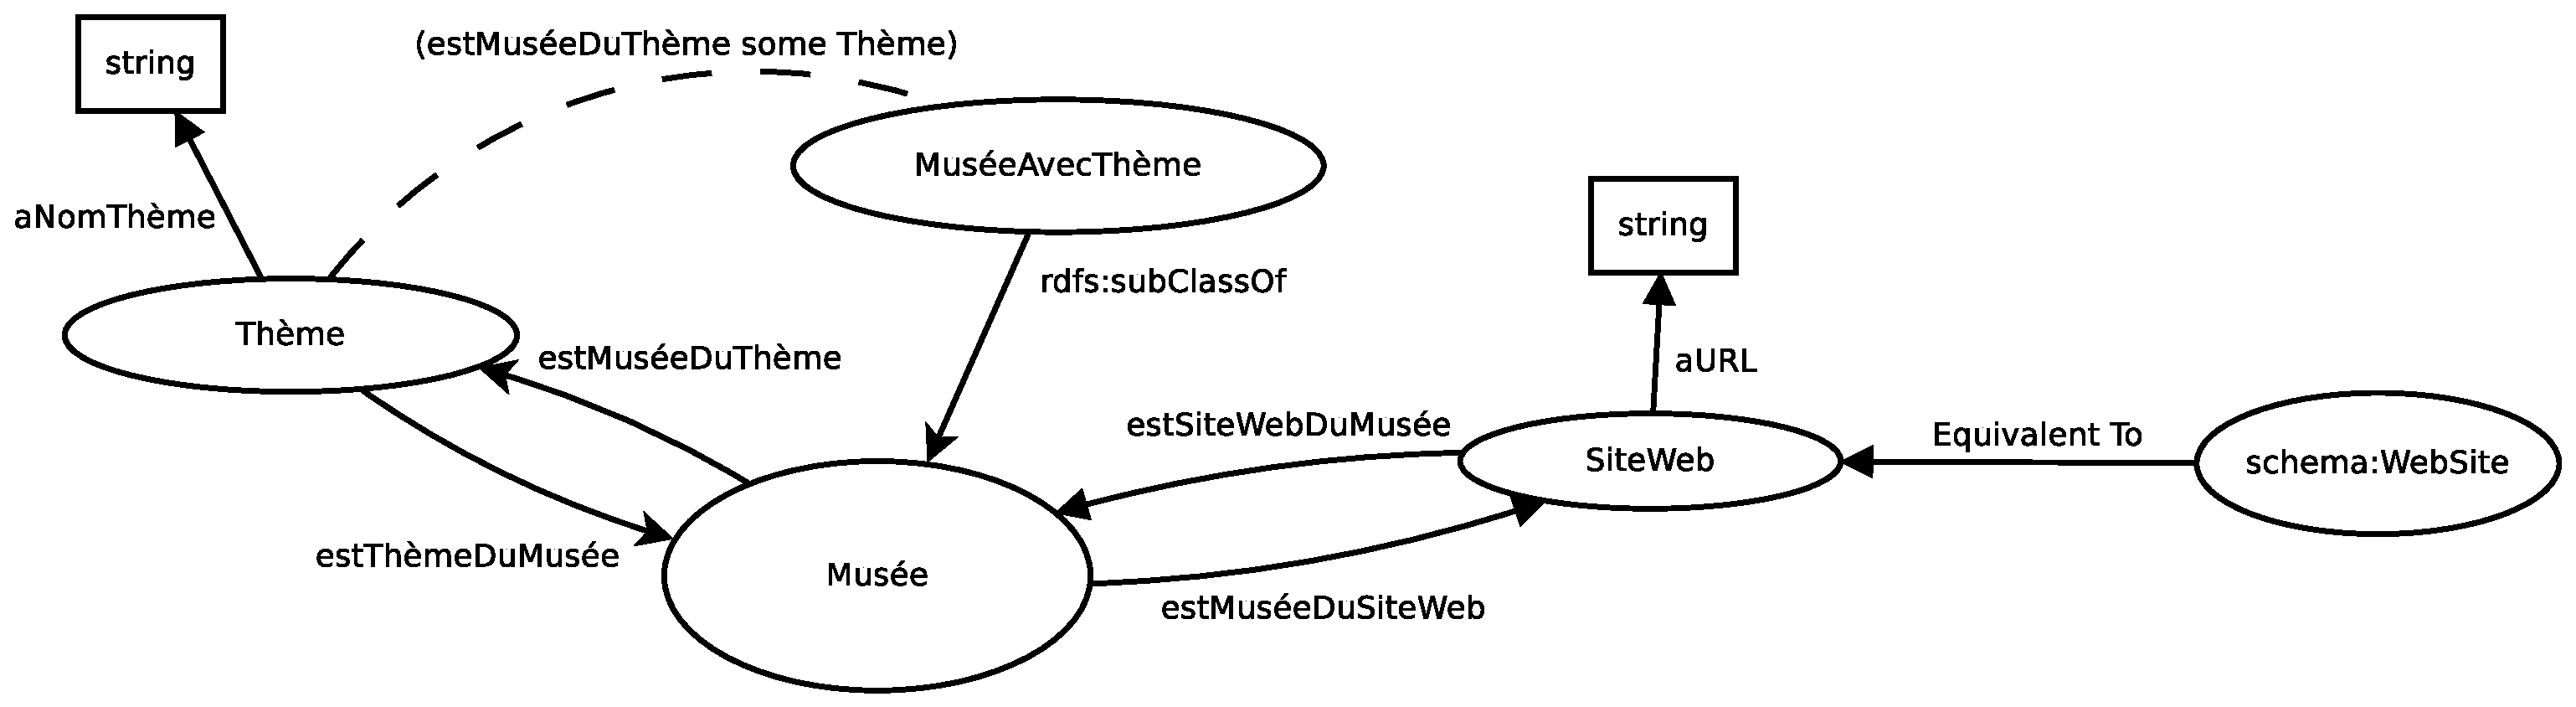
\includegraphics[width=16cm]{Diagramme2.eps}
\end{center}
\vspace{0.3cm}
\begin{center}
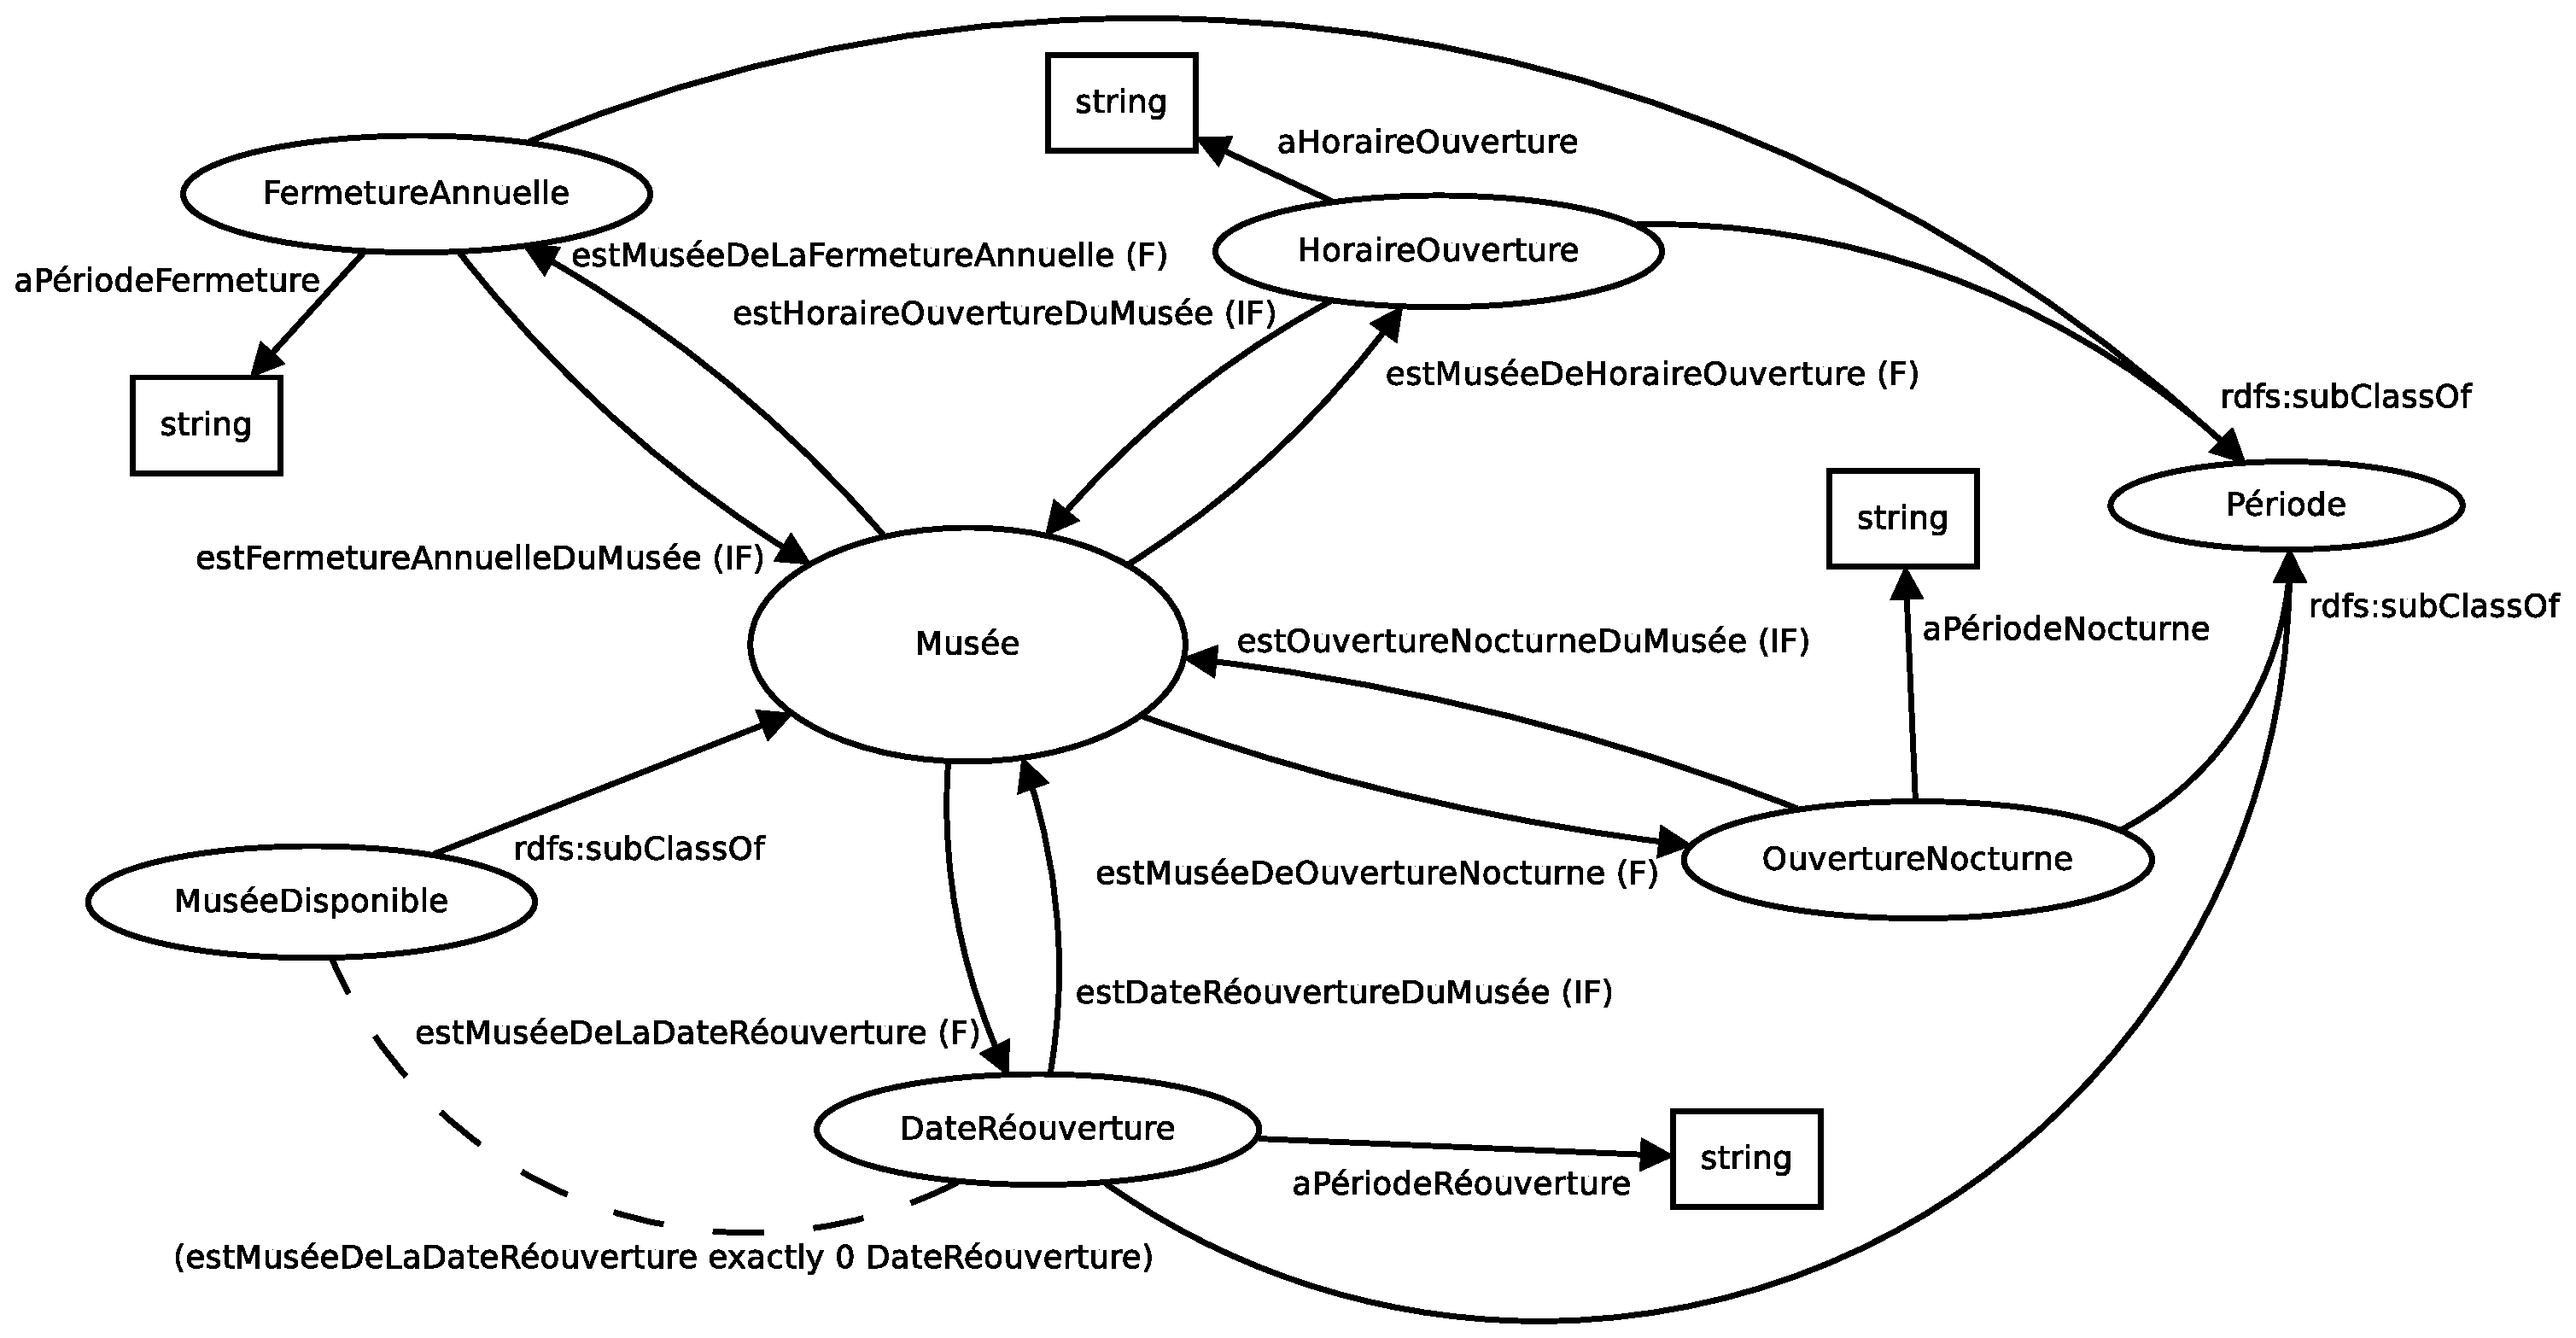
\includegraphics[width=16cm]{Diagramme3.eps}
\end{center}

\subsection{Importation des données}

\subsubsection{Génération via un programme Java}

\subsubsection{Inférences dans protege}

\section{Partie 2 : Intégration de l'ontologie dans une application Java}

\subsection{Type de l'application}

\subsection{Fonctionnalités}

\subsubsection{Recherche}

\subsubsection{Fiche Région (DBPedia)}

\subsubsection{Localisation (Google MAP)}

\section{Répartition du travail}


\end{document}